\begin{figure*}[htbp]
    \centering
    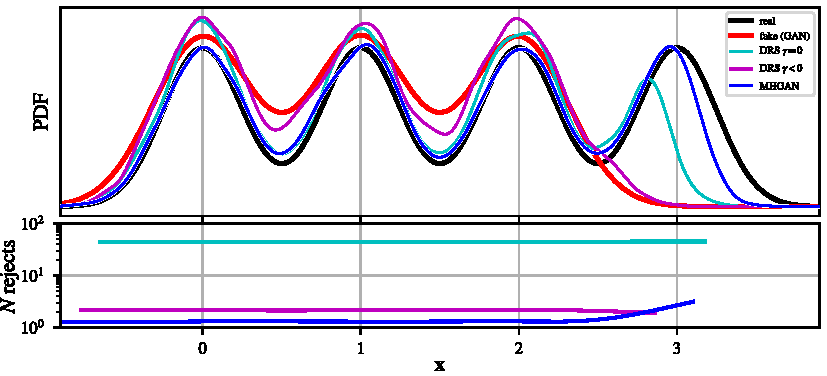
\includegraphics[width=1.0\linewidth]{figures/univariate_example_flat.pdf}
    \caption{{\small
    Illustration comparing the MH-GAN setup with the formulation of DRS on a univariate example.
    This figures uses a $\PR$ of four Gaussian mixtures while $\PG$ is missing one of the mixtures.
    The top row shows the resulting density of samples, while the bottom row shows the typical number of rejects before accepting a sample at that $\vec x$ value.
    The MH-GAN recovers the true density except in the far right tail where there is an exponentially small chance of getting a sample from the proposal $\PG$.
    DRS with $\gamma=0$ shift should also be able to recover the density exactly, but it has an even larger error in the right tail.
    These errors arise because we must approximate the max $D$ score and use only \num{10000} pilot samples to do so, as in \citet{Azadi2018}.
    Additionally, due to the large maximum $D$, it needs a large number of draws before a single accept.
    DRS with $\gamma$ shift is much more sample efficient, but completely misses the right mode as the setup invalidates the rejection sampling equations.
    The MH-GAN is more adaptive in that it quickly accepts samples for the areas $\PG$ models well; more MCMC rejections occur before accepting a sample in the right poorly modeled mode.
    In all cases the MH-GAN is more efficient than DRS without $\gamma$ shift.
    Presumably, this effect becomes greater in high dimensions.
    }}
    \label{fig:univariate_example}
\end{figure*}
